\section{VANET}
    VANET(Vehicle Ad-hoc Network)는 ITS의 핵심 기술 중 하나로, 도로 위 움직이는 다수의 차량들이 무선통신을 이용하여 차량 간 통신 또는 차량과 도로변 인프라 장치간의 통신을 제공하는 차세대 네트워킹 기술이다. VANET은 이동성이 높은 차량의 특성을 이용하여 각 차량이 별도의 기지국과 통신하는 대신에 차량과 차량(V2V, Vehicle to Vehicle), 차량과 도로변 인프라 장치(V2I, Vehicle to Infrastructure)가 연결된 자율인 네트워크를 구성한다. 각 차량은 VANET를 통해 교통 혼잡, 교통 사고, 도로 표면 상태 등 여러 교통 정보를 공유한다. \\
    \vspace{-4mm}
    \begin{figure}[!h]\centering
		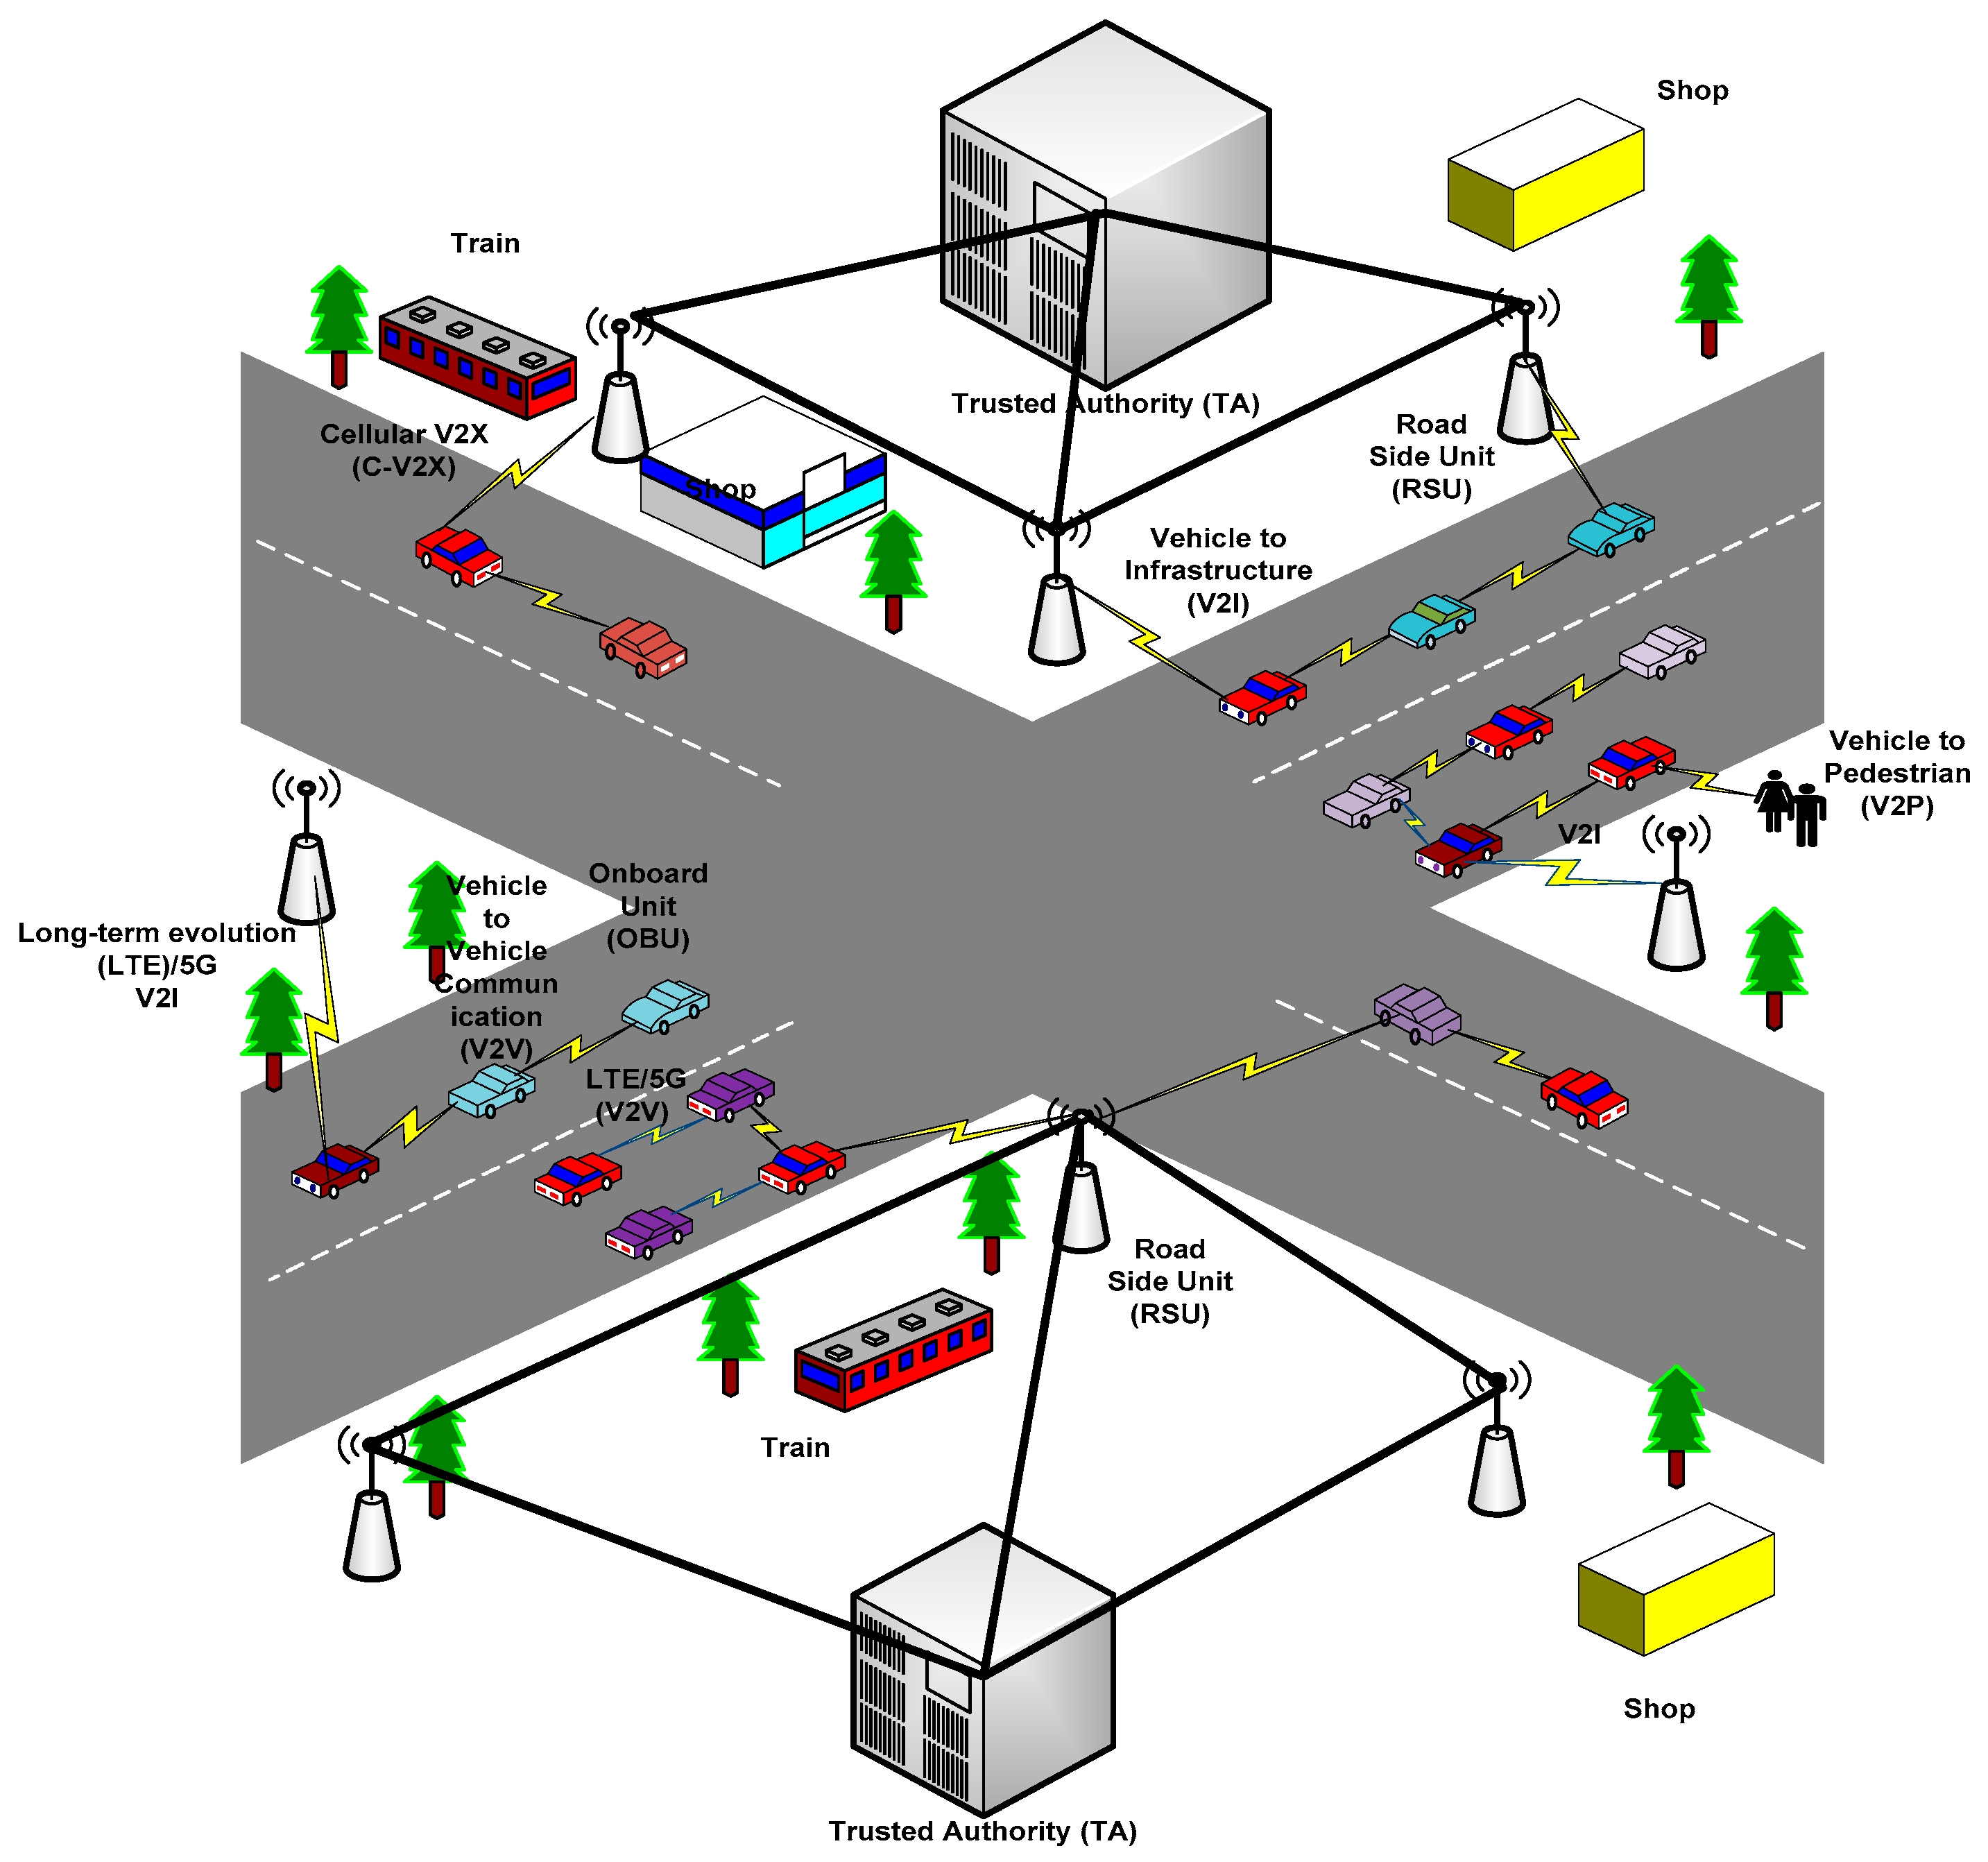
\includegraphics[width=.65\textwidth]{image/week13/2-1.png}
		\caption{\small VANET(Vehicle Ad-hoc Network)}
		\vspace{-10pt}
    \end{figure}